\chapter{Conclusions}
This chapter tries to summarize what was learned during those 5 months. Also a critical self-reflection of the author is included.

\paragraph{Looking back}
When I look back about 5 months, I certainly have seen myself grow in the subject. Even though I was not very new to the subject matter, I did discover a bunch of new material that was very interesting to get my hands dirty on. Going to the deep internals of Apache Solr and writing a plugin might have been the most challenging one, all the other tasks required a lot of patience and a good ear and eye for community feedback. Although I do feel I should discover more and alternate technologies and get a broader knowledge of what is available in the field.
An approximate amount of 1000 man-hours was spend working on this subject, and I'm happy to work a bunch more of them on this same topic. 
On another matter I am still very much convinced that open source is the way to go in writing code that is used for the general public. Knowing that more than 10000 people use your code, and also care enough to give feedback and even improving the code is a very good sign. People evolve, and so does code. I'm sure that when I look back in a  year to the same codebase it won't be the same anymore, and happily so! Improving yourself is also an important process in the learning curve and as everyone in this sector one should keep learning or you'll fall behind. 

\section{Reflection on Apache Solr}
Apache Solr is a very powerful layer build upon Apache Lucene, I have had the pleasure to work with Solr for the past 5 months very intensively and it has almost never let me down. It has some flaws, such as not supporting the Near Realtime Search, but it will overcome those in the near future hopefully. Also, having other projects like Elastic Search in the same corner is a benefit for Apache Solr. I wouldn't consider them competition because the only software that Apache Solr is competing with are highly licensed software products that lack in transparency. Software like the Google Search Appliance, but also software such as Microsoft fast are a direct prey for open source applications. 
I hope to see much more development in this field and I'm sure that my contributions have helped Acquia in improving their search farm.

\section{Reflection on Drupal 6 and Drupal 7 in regards to search integration}
Drupal has been one of my favorite projects in the last couple of years. I could only dream of being able to contribute such an amount of time to the project. By taking up this challenge of having my thesis semester at Acquia I could also realize that dream. I've seen the amount of websites that use the Apache Solr Module grow during my internship from 9000 to around 11000 websites. The Apache Solr 7 module even had a more spectacular growth coming from 1400 to 3050 websites. It has more than doubled its user base. As one of the maintainers, together with a bunch of other people in the community, I am very proud to see such a growth.
It can only be concluded that it means that the community, Acquia and I did a good job in improving the module and there is still a bunch of work to be done!

\section{Timeline}
\begin{figure}[H]
     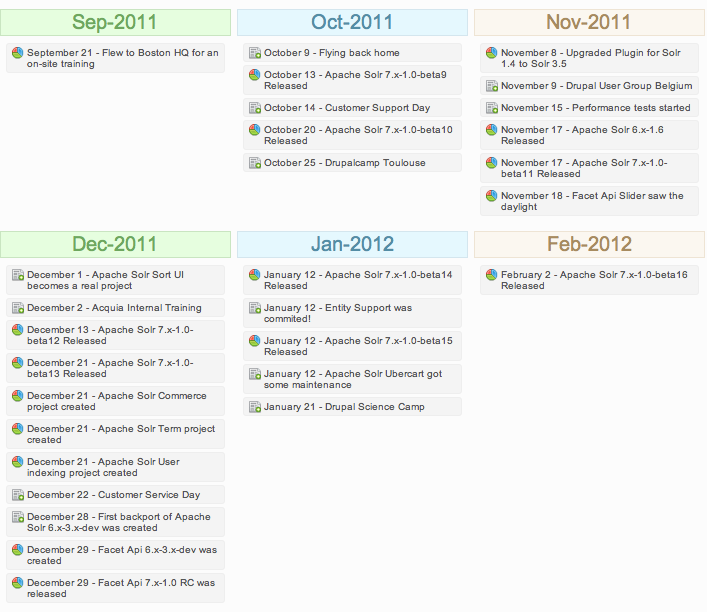
\includegraphics[width=\textwidth]{images/event_timeline.png}
     \caption{A graphical representation of the actions that occured during my internship. A dynamic version can be found on \url{http://timeline.nickveenhof.be/}}
\end{figure}


\section{Future Work}
\subsection{Apache Solr Search Integration}
Drupal 7 has made a significant improvement in regards of its search functionality. By default, Drupal hardly ships with a good search engine but it does allow contributed modules to plug into the core system of Drupal and completely overtake the search functionality. The Search API module makes very good use of this system and it seems that this project has a good chance of replacing (or at least a small amount of it) the current code in Drupal core 8 or later. Even if that does not happen, a motivated amount of people are ready to take the next step to keep on improving search in Drupal and as a consequence also future modules. wether this is an integration with Apache Solr or another open source search engine, the important part is that people stay motivated to keep improving the code and themselves. As an individual, as an employee, and as a student I am still very motivated to keep working on Drupal, the integration with search, myself and who knows what else. The best is yet to come!

\subsection{Acquia Search}
Acquia Search is a wonderful piece of work that was created for Apache Solr 1.4 when it first found its offspring. Every subscription that acquia opens ships with search as a service for that subscription's Drupal website. Being able to work with a service that has a massive impact and even being able to know that clients depend on the work you've done and within the timeframe of your internship launch a website that utilizes your work is very pleasant and rewarding.

\chapter{Feedback from the mentors at Acquia}
In a recommendation of my mentor Carles Farré I have included feedback from the company into this work.

\section{Chris Brookins}
Nick Veenhof worked for Acquia as an intern between October 2011 and Feb 2012.  Acquia is a commercial open source software company providing products, services, and technical support for the open source Drupal social publishing system.  In that time he contributed significantly to our Acquia Search web service \footnote{\url{http://www.acquia.com/products-services/acquia-network/cloud-services/acquia-search}} and to the Drupal modules that work with any Apache Solr instance including the \url{http://drupal.org/project/apachesolr} and url{http://drupal.org/project/facetapi}.  These modules are GPL and are available to anyone using the Drupal open source project. Nick did outstanding work, contributing to the following project milestones and working as needed with other Acquia engineers.

\begin{packed_itemize}
\item Enhance the Apachesolr 7.x-1.x project to the RC1 stage
\item Enhance the Facetapi 7.x-1.x project to RC1 stage
\item Create the Apachesolr 6.x-3.x, and get it to beta1 stage
\item Create the Facetapi 6.x-3.x, and get to beta1 stage
\item Ported our Java code for client authentication to work with Solr 3.5
\item Upgrade an cluster of the Acquia Search service to Solr 3.5 in order to support a beta test customer
\item Develop and run load tests to compare Solr 1.4.1 and Solr 3.5 on our servers
\end{packed_itemize}
Nick needed a minimal amount of guidance and direction and took strong initiative in all of these projects. His work will enhance both the Drupal project and our product offering that supports thousands of customers and millions of search requests.

\section{Peter Wolanin}
I had the role of technical mentor and the most direct supervisor for
Mr. Nick Veenhof during his internship from October 2011 and Feb 2012.
Throughout most of this period Mr. Veenhof and I had nearly daily
calls to plan and discuss his work.

Mr. Veenhof came into the project already familiar with the Drupal 7
core APIs, but without a lot of a in-depth experience with the Apache
Solr Search Integration module that was the focus of his work. He
rapidly became very productive in improving and extending the code of
this module, and it was a pleasure to be able to formulate a plan with
him and meet again the next day to find a well-executed
implementation.

I was particularly impressed with Mr. Veenhof's independence and
initiative in two areas.  First, he re-organized the administrative
user interface for the module through an iterative process and brought
it much more in line with Drupal 7 standards. Later, during January,
he moved ahead and made initial Drupal 6 backports of the working
Drupal 7 versions of the Apache Solr Search Integration and Facet API
modules.

In addition to the work on the Drupal module, Mr. Veenhof adapted our
existing servlet filter code that does authentication so it worked
with the latest Solr 3.5 release.  The Solr codebase had been
reorganized, so our build and integration no longer worked.  We had
expected to have to hire an outside consultant, but Mr. Veenhof
researched the problem and was able to solve the problem himself. He
further invested significant time validating that the Drupal
integration module worked correctly with this new version of Solr, and
doing comparative performance benchmarks between Solr 3.5 and 1.4 to
validate our planned upgrade.

Mr. Veenhof has also gone above and beyond by communicating the
results of his development efforts to the larger Drupal community by
presenting his work at Drupal events and through technical blog posts,
neither of which were a required part of his internship.

There were very few areas where Mr. Veenhof needed any improvement.
On occasion, perhaps, Mr. Veenhof needed to be pushed to reconsider
his implementation approach or to backtrack and understand in more
depth the algorithm he was trying to modify.  I would consider this
mostly a reflection of his enthusiasm to move ahead in the project.

Overall, I consider his internship as tremendously productive. It
delivered improvements to the open-source code as well as to Acquia's
internal systems, and gave Mr. Veenhof the chance to become one of the
leading experts in this area.

Peter Wolanin, Ph.D.
Principal Engineer, Acquia, Inc.